% !TEX encoding = UTF-8
% !TEX program = xelatex

\documentclass[10.5pt]{myarticle}

\usepackage{lecturenoteStyle_2023}

\title{\bf 大作业报告——图像去噪的 K-SVD 算法}
\author{李梓健、孙天一、檀嘉宸、王子赫、张绍轩}
\date{}

\begin{document}
	
\maketitle

\section{算法介绍}

\subsection{优化算法:K-SVD 算法}
K-SVD(K-Singular Value Decomposition)是一种高效的字典学习算法,用于信号重建和降噪。它通过迭代过程优化过完备字典,以更好地表示输入数据。在图像降噪中,K-SVD旨在找到一个稀疏表示,该表示能够最小化重建误差并保留图像的重要特征。

K-SVD 算法的一般流程如下:
\begin{enumerate}
	\item 初始化:使用初始预定义字典进行初始化;
	\item 稀疏编码:对每个图像块应用稀疏编码,以找到其在当前字典下的最佳表示;
	\item 字典更新:对每个字典元素,使用恰当更新方法来最小化重建误差;
	\item 迭代:重复稀疏编码和字典更新步骤,直到满足收敛条件. 
\end{enumerate}

在本项目中,我们采用 DCT 过完备字典作为初始字典;利用 OMP(正交匹配追踪)算法进行系数编码;在字典更新中,利用最速下降法最小化残差来更新字典元素.
 
\begin{algorithm}[H]
	\caption{K-SVD}
	\label{alg:ksvd}
	
	\KwIn{$X$: the patches}
	\KwOut{$D$: the learned dictionary, $A$: the sparse representation}
	
	$D_0 \gets \mathrm{DCT}_{2N}$ \tcp*{the initial overcomplete dictionary}
	\For{$i = 0$ \KwTo max\_iter}{
		\If{$i > 0$}{
			$D_i \gets \text{DictLearn}(X, A)$
		}
		$A_i \gets \text{OMP}(X, D)$
	}
\end{algorithm}

\subsubsection{初始字典:DCT 过完备字典}
DCT(离散余弦变换)是一种常用于信号处理和图像压缩的变换方法.  对于初始图像样本 $X$,DCT 可以将图像转换成在频域中表示的系数. 

DCT 过完备字典是 K-SVD 算法中常用的初始字典,它包含了DCT基础上的各种变体和组合. 这样的字典提供了一个良好的起点,可以捕捉图像数据中的多种特征.

构建过程:
\begin{enumerate}
	\item 选择 DCT 基: 根据块的规模 $N$,选取 $N$ 阶 DCT 变换矩阵作为初始 DCT 基. 
	\begin{align*}
		\mathcal{C} = \left( \cos \left(\frac{2\pi}{N} jk\right) \right)_{j, k = 1, \cdots, N}
	\end{align*}
	
	\item 构造过完备字典: 利用以下规则扩展基元素
	\begin{align*}
		D = \mathcal{C} \otimes \left( \cos \frac{2\pi}{2N} j(2k-1), 1 \right)
	\end{align*}
	
	这相当于对一个 $2N$ 阶 DCT 变换矩阵进行裁切. 
	\item 归一化: 将字典元素归一化,以避免数值问题. 
\end{enumerate}

\subsubsection{稀疏编码:OMP 算法}
OMP(正交匹配追踪)是一种贪婪算法,用于在给定字典的情况下找到信号的稀疏表示。在K-SVD中,它用于确定每个图像块的稀疏系数. 

设输入信号为 $x$,字典为 $D$,OMP 算法的目标是在满足稀疏度的前提下,寻找最优的稀疏表示. 这里最优性是指
\begin{align}
	\min |x - Da|_2
\end{align}

在本项目中,我们对每条信号(即每个 patch )都执行 OMP 算法,从而确定整体的稀疏编码 $A: X \approx DA$. 

\begin{algorithm}[H]
	\caption{Orthogonal Matching Pursuit}
	\label{alg:omp}
	
	\KwIn{$x$: a single signal, $D$: the dictionary, $s$: sparsity}
	\KwOut{$a_x$: the sparse representation of $x$}
	
	$a_x = 0$, $r = x$ \tcp*{Initialization}
	\While{$|x|_0 \leq s$}{
		$k = \arg\max_j \{d_j^T r: d_j \text{ is the } j^{\text{th}} \text{ column of } D \}$ \\
		$x_k += d_k^T r$ \tcp*{Update}
		$r -= d_k^T r \cdot d_k$ \\
		\If{$|r|_2 < \varepsilon$}{
			break
		}
	}
\end{algorithm}

\subsection{字典学习方法}
字典更新是 K-SVD 算法中的核心步骤,目的是优化字典以更好地适应数据. 我们采用的字典更新原则如下: 

~

\begin{enumerate}
	\item 选取字典中的原子: 对于每一个字典中的原子(基向量),依次进行更新. 设当前从字典中选择原子 $d_k$. 
%	\item 对于当前待更新的原子,找到使用该原子进行稀疏编码的样本。
%	
%	设 $ I_k = \{ j: x_jk \neq 0 \} $,令 $ Y_k = Y_{I_k} $ 表示使用原子 $d_k$ 进行稀疏编码的样本,$X_k = X_{I_k \times k} $ 表示相应稀疏编码的系数.
%	
%	\item 通过梯度下降法优最小化残差,以更新当前选定的原子. 这里优化目标为
%	\begin{align}
%		\min_{d_k \in \mathbb{R}^{\mathrm{P}}} \Phi(d_k) = \frac{1}{2} \| Y_k - d_k X_k \|_F^2
%	\end{align}
%	
%	% 其中 $ \nabla \Phi (d_k) = - (Y_k - d_k X_k) X_k^T $
%	\item 重复迭代: 对所有字典中的原子重复步骤 1-3,直到满足停止条件(如达到最大迭代次数或字典变化不大)
\end{enumerate}

以下是从灰色图像中学习到的字典结果

%\begin{figure}[H]
%	\centering
%	\subfloat[Barbara]{ 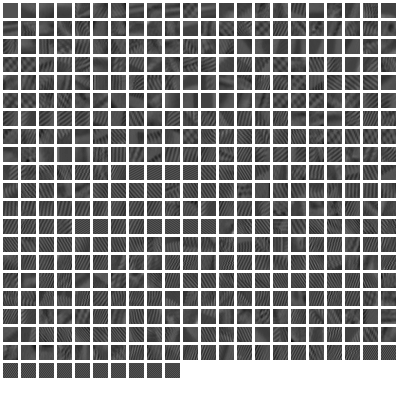
\includegraphics[width=55mm]{../results/dictionaries/barbara_512.png} }  
%	\subfloat[Cameraman]{ 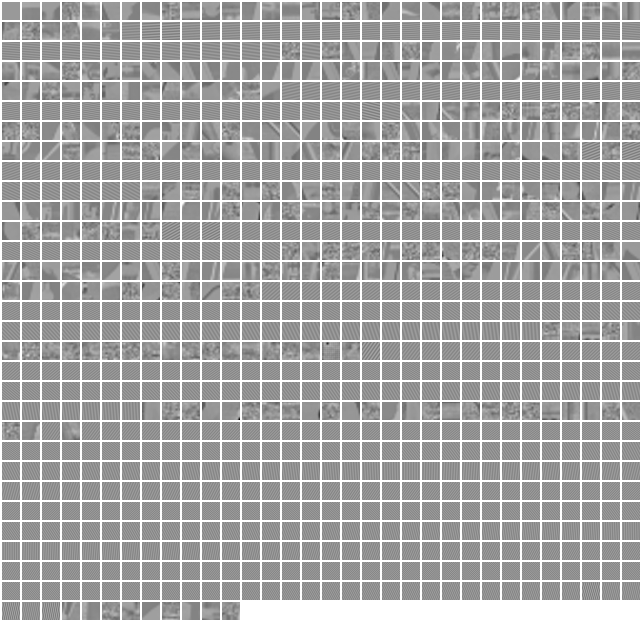
\includegraphics[width=55mm]{../results/dictionaries/cameraman_512.png} }  
%	\subfloat[Lena]{ 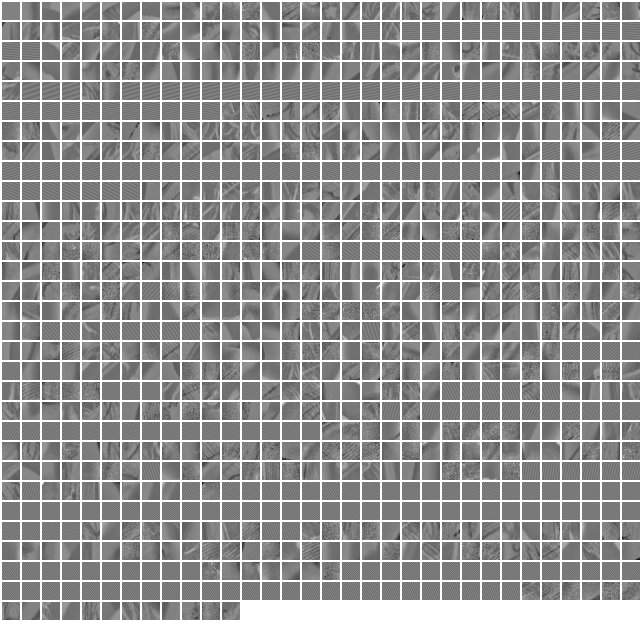
\includegraphics[width=55mm]{../results/dictionaries/lena_512.png} }  \\ 
%	\caption{Dictionary learned from three grayscale images.}
%	\label{fig:dl_gray}
%\end{figure}

%\begin{remark}
%	The above contents are basically ``Task 1''.
%\end{remark}

\section{数值结果}

各个任务的数值结果展示如下:

\subsection{Task 3: 彩色图像学习}

对于彩色图像,使用清晰图像进行字典学习与图像降噪,PSNR结果如表 \ref{tab:result_task3} 所示

\begin{table}[H]
	\centering
	\caption{PSNR values of 18 McM images.}
	\label{tab:result_task3}
	\begin{tabular}{|c|c|c|c|c|}
		\hline
		 & Red Channel & Green Channel & Blue Channel & Average of three \\ \hline
		McM01 & 27.04  & 27.26  & 27.66  & 27.32  \\ \hline
		McM02 & 30.79  & 32.34  & 31.94  & 31.69  \\ \hline
		McM03 & 25.55  & 25.81  & 25.03  & 25.46  \\ \hline
		McM04 & 27.90  & 29.58  & 27.32  & 28.27  \\ \hline
		McM05 & 31.23  & 29.63  & 28.83  & 29.90  \\ \hline
		McM06 & 30.63  & 30.08  & 31.00  & 30.57  \\ \hline
		McM07 & 29.79  & 30.52  & 30.20  & 30.17  \\ \hline
		McM08 & 34.00  & 34.52  & 34.36  & 34.29  \\ \hline
		McM09 & 31.05  & 32.60  & 33.39  & 32.35  \\ \hline
		McM10 & 32.10  & 32.56  & 32.99  & 32.55  \\ \hline
		McM11 & 32.20  & 32.39  & 34.76  & 33.11  \\ \hline
		McM12 & 34.27  & 33.95  & 34.03  & 34.08  \\ \hline
		McM13 & 35.07  & 34.80  & 33.83  & 34.57  \\ \hline
		McM14 & 34.78  & 34.87  & 33.96  & 34.53  \\ \hline
		McM15 & 33.79  & 34.61  & 34.91  & 34.44  \\ \hline
		McM16 & 24.50  & 23.06  & 29.94  & 25.83  \\ \hline
		McM17 & 25.30  & 27.58  & 28.49  & 27.12  \\ \hline
		McM18 & 27.49  & 27.82  & 32.30  & 29.21  \\ \hline
	\end{tabular}
	%
\end{table}

作为对比,噪声图像的 PSNR 结果如表 \ref{tab:noisy_task3} 所示. 

\begin{table}[H]
	\centering
	\caption{PSNR values of 18 noised McM images.}
	\label{tab:noisy_task3}
	\begin{tabular}{|c|c|c|c|c|}
	\hline
		 & Red Channel & Green Channel & Blue Channel & Average of three \\ \hline
		McM01 & 22.10 & 22.08 & 22.12 & 22.12 \\ \hline
		McM02 & 22.09 & 22.12 & 22.12 & 22.12 \\ \hline
		McM03 & 22.11 & 22.12 & 22.11 & 22.11 \\ \hline
		McM04 & 22.10 & 22.12 & 22.14 & 22.14 \\ \hline
		McM05 & 22.11 & 22.10 & 22.12 & 22.12 \\ \hline
		McM06 & 22.10 & 22.11 & 22.12 & 22.12 \\ \hline
		McM07 & 22.10 & 22.12 & 22.13 & 22.13 \\ \hline
		McM08 & 22.10 & 22.12 & 22.11 & 22.11 \\ \hline
		McM09 & 22.11 & 22.11 & 22.09 & 22.09 \\ \hline
		McM10 & 22.10 & 22.13 & 22.12 & 22.12 \\ \hline
		McM11 & 22.12 & 22.11 & 22.11 & 22.11 \\ \hline
		McM12 & 22.13 & 22.11 & 22.10 & 22.10 \\ \hline
		McM13 & 22.10 & 22.09 & 22.12 & 22.12 \\ \hline
		McM14 & 22.11 & 22.10 & 22.10 & 22.10 \\ \hline
		McM15 & 22.12 & 22.10 & 22.13 & 22.13 \\ \hline
		McM16 & 22.09 & 22.09 & 22.11 & 22.11 \\ \hline
		McM17 & 22.11 & 22.11 & 22.10 & 22.10 \\ \hline
		McM18 & 22.12 & 22.12 & 22.13 & 22.13 \\ \hline
	\end{tabular}
	%
\end{table}


\clearpage


\subsection{Task 4: 未知清晰图像情形}

\begin{table}[H]
	\centering
	\caption{PSNR values of 18 McM images.}
	\label{tab:result_task4}
	\begin{tabular}{|c|c|c|c|c|}
		\hline
		 & Red Channel & Green Channel & Blue Channel & Average of three \\ \hline
		McM01 &  &  &  &  \\ \hline
		McM02 &  &  &  &  \\ \hline
		McM03 &  &  &  &  \\ \hline
		McM04 &  &  &  &  \\ \hline
		McM05 &  &  &  &  \\ \hline
		McM06 &  &  &  &  \\ \hline
		McM07 &  &  &  &  \\ \hline
		McM08 &  &  &  &  \\ \hline
		McM09 &  &  &  &  \\ \hline
		McM10 &  &  &  &  \\ \hline
		McM11 &  &  &  &  \\ \hline
		McM12 &  &  &  &  \\ \hline
		McM13 &  &  &  &  \\ \hline
		McM14 &  &  &  &  \\ \hline
		McM15 &  &  &  &  \\ \hline
		McM16 &  &  &  &  \\ \hline
		McM17 &  &  &  &  \\ \hline
		McM18 &  &  &  &  \\ \hline
	\end{tabular}
\end{table}

\clearpage

\section{总结}

\end{document}



